\chapter{Potencial generalizado. Campo electromagnético}
\label{T7PotenGener}

	
\begin{tikzpicture}
	\fill [left color=red!50, right color=teal!50] (0,0) rectangle (6.5,.1);
	\fill [left color=teal!50, right color=blue!50] (6.5,0) rectangle (11.5,.1);
	\end{tikzpicture}


\vspace{10mm}
\begin{adjustwidth}{50pt}{50pt}
\begin{ejemplo}
	Vamos a introducir el \emph{potencial generalizado} aplicado a la fuerza de Lorentz no relativista, $\ \overrightarrow F  =  q \ (\overrightarrow E + \vec v \times \overrightarrow B)\ $. Nuestro objetivo será la formulación del lagrangiano con un cierto potencial $U(q,\dot q,t)$ que responda a la presencia de campos electromagnéticos. ($U$ no solo dependerá de las posiciones $q$ sino también de la velocidades $\dot q$ y del tiempo $t$).
\end{ejemplo}
\end{adjustwidth}


\section{Potencial generalizado}
\vspace{5mm}

La definición de potencial generalizado va a ser:

\begin{equation}
\label{T7potengener}
U(q,\dot q, t) \quad / \qquad \quad \boldsymbol{ Q_j \ = \ \dv{t} \left[ \pdv{U}{\dot q_j} \right] \ - \ \pdv{U}{q_j} }	
\end{equation}


El potencial generalizado $U$ ha de ser una función tal que una fuerza generalizada $Q_j$ se pueda escribir de este modo (Euler-Lagrange) en función de esta $U$, así, el potencial generalizado dará lugar a la fuerza generalizada.

Veamos un ejemplo:

\begin{example}
	\textbf{\emph{Acoplamiento mínimo}} (mecánica cuántica): un electrón en un átomo de Hidrógeno se encuentra sometido a radiación electromagnética externa. Hablaremos de ello al final del tema.	
\end{example}

\vspace{10mm}
\ul{Inciso-1} $\quad$ \rule{100pt}{0.1pt} $\quad$ \textbf{Regla mnemotécnica para el producto vectorial.}

$\vec a\times \vec b=\vec c \ \to \ 
\begin{cases}
\ c_1=a_2b_3-a_3b_2 \\ \  c_2=a_3b_1-a_1b_3 \\  \ c_3=a_1b_2-a_2b_1 	
\end{cases} \qquad \text{orden: } 1231231\cdots \ ,\ $ 

después del 1 va el 2, después el 3, luego el 1 de nuevo y así. Para la componente 3 del producto vectorial, por ejemplo, después de 3 vuelve el 1 y el 2, por eso aparece $a_1b_2$ y luego, restando, al revés, $a_2b_1$.

\vspace{-5mm}

\begin{flushright}
\rule{300pt}{0.1pt}	
\end{flushright}



Aplicado al producto $\ \vec v \times \overrightarrow B \ = \ 
(v_2B_3-v_3B_2,\ v_3B_1-v_1B_3,\ v_1B_2-v_2B_1)$

Y la fuerza de Lorentz, $\ \overrightarrow F \ = q\ \vec B \times \overrightarrow B \, $:

\begin{equation}
\label{T7Lorentz}
\begin{split}
F_1 = q(E_1+v_2B_3-v_3B_2)	\\
F_2 = q(E_2+v_3B_1-v_1B_3)	\\
F_3 = q(E_3+ v_1B_2-v_2B_1)
\end{split}	
\end{equation}

\vspace{5mm}%10
\ul{Inciso-2} $\quad$ \rule{150pt}{0.1pt} $\quad$ \textbf{Teoremas de Cálculo Vectorial.}

\begin{theorem}
.	\vspace{2mm}

	\textbf{Teorema 1} \hspace{2cm} $\qquad \boldsymbol{ \overrightarrow \nabla \cdot (\overrightarrow \nabla \times \overrightarrow A) = 0 } \, ,\quad \forall \overrightarrow A$ 
	
	\vspace{2mm} \textbf{Teorema 2} \hspace{2cm} $\qquad \boldsymbol{ \overrightarrow \nabla \times (\overrightarrow \nabla \ f) = 0 } \, ,\quad \forall \overrightarrow f$ 
	
	\vspace{3mm} \textcolor{gris}{Th1: La divergencia del rotacional es cero.  \hspace{1cm} Th2: El rotacional del gradiente es cero.}
	
	\vspace{2mm}
\end{theorem}

\vspace{-5mm}
\begin{proof} (Primer teorema).

Llamando $\displaystyle \ \partial_1 = \pdv{x}\, , \ \ \partial_2 = \pdv{y}\, , \ \ \partial_3 = \pdv{z} \, , \ $ podemos escribir

$\overrightarrow \nabla \times \overrightarrow A = (\partial_2A_3-\partial_3A_2 , \ \partial_3A_1-\partial_1A_3 , \ \partial_1A_2 - \partial_2A_1)$

$\overrightarrow \nabla \cdot \overrightarrow \nabla \times \overrightarrow A = 
(\partial_1 , \partial_2 , \partial_3 ) \cdot 
(\partial_2A_3-\partial_3A_2 , \ \partial_3A_1-\partial_1A_3 , \ \partial_1A_2 - \partial_2A_1)=$

$\overrightarrow \nabla \cdot \overrightarrow \nabla \times \overrightarrow A =  \partial_1 (\partial_2A_3-\partial_3A_2 ) + \partial_2 ( \partial_3A_1-\partial_1A_3 ) +\partial_3 (\partial_1A_2 - \partial_2A_1)=$

Teniendo en cuenta el teorema de Schwartz, para funciones derivables con derivada continua podemos intercambiar el orden de las derivadas parciales, por ejemplo, $\partial_1 \partial_2 A_3 = \partial_2 \partial_1 A_3$, tendremos, 

$\overrightarrow \nabla \cdot \overrightarrow \nabla \times \overrightarrow A = \cancel{\partial_1 \partial_2A_3} - \bcancel{\partial_1 \partial_3A_2 } + \underline{\partial_2  \partial_3A_1}- \cancel{\partial_2 \partial_1A_3 } + \bcancel{\partial_3 \partial_1A_2} - \underline{\partial_3  \partial_2A_1}= 0$
	
\end{proof}

\vspace{-13mm}

\begin{flushright}
\rule{300pt}{0.1pt}	
\end{flushright}

\vspace{10mm}

Para nuestro propósito vamos a necesitar 3 de las 4 ecuaciones de Maxwell (la cuarta es necesaria para describir ondas electromagnéticas, pero no es nuestro caso).

\begin{small}\textcolor{gris}{No hay distribución de cargas, $\rho=0 \ \to \ \overrightarrow \nabla \cdot E =0$, hay una onda \emph{em} plana que afecta a nuestra carga q.}\end{small}

\begin{myblock}{Ecuaciones de Maxwell (3/4)}
\begin{Large}
\begin{equation} \boldsymbol{
\overrightarrow \nabla \cdot \overrightarrow E = 0\, ; \quad  \quad \overrightarrow \nabla \cdot \overrightarrow B = 0\, ; \quad  \quad \overrightarrow \nabla \times \overrightarrow E = - \pdv{\overrightarrow B}{t} }
\end{equation}
\end{Large}
\end{myblock}

\vspace{5mm}
\normalsize{Nuestro} \underline{objetivo} va a ser encontrar cuatro cantidades $A_0,\ A_1,\ A_2, \ A_3$ (función) de modo que cuando la derivemos con respecto a $x,y,z,t$ nos proporcione los campos $\overrightarrow E$ y $\overrightarrow B$. A estas cuatro cantidades $A^\mu=(A_0, A_1, A_2, A_3)=(A_0,\  \overrightarrow A)$, que dependen de $x,y,z,t$ forma un \emph{cuadrivector} que llamaremos \textbf{Potencial Vector}, $\boldsymbol{A^\mu}$. A partir de combinaciones de derivadas de $A^\mu$ queremos obtener $\overrightarrow E$ y $\overrightarrow B$.

\vspace{5mm} Como la divergencia del rotacional es cero, $\ \overrightarrow \nabla \cdot (\textcolor{red}{\overrightarrow \nabla \times \overrightarrow A})=0\ $ (teorema-1), si nos fijamos en la segunda de Maxwell, M2, $\ \textcolor{red}{\overrightarrow \nabla \cdot B} =0 \, , \  $ concluimos que debe ocurrir que:

\begin{equation}
\textcolor{red}{\boldsymbol{ \overrightarrow B \ = \ \overrightarrow \nabla \cdot \overrightarrow A }}	
\end{equation}
 
 Falta trabajar con las otras dos ecuaciones de Maxwell, M1 y M3.
 
 Si nos fijamos en M3: $ \qquad \overrightarrow \nabla \times \overrightarrow E = \displaystyle -\pdv{t} \ \textcolor{red}{\overrightarrow B} = -\pdv{t} ( \textcolor{red}{\overrightarrow \nabla \times \overrightarrow A })$
 
 Podemos conmutar la derivación por el teorema de Scwartz,: $\quad \displaystyle - \pdv{t} ( \overrightarrow \nabla \times \overrightarrow A ) = - \overrightarrow \nabla \times \left( \pdv{\overrightarrow A}{t}  \right)$
 
 Pasando a la izquierda, $\quad \displaystyle \overrightarrow \nabla \times E \ + \  \overrightarrow \nabla  \times \left( \pdv{\overrightarrow A}{t}  \right) = 0 \, , \ $ agrupando, $\quad \displaystyle \overrightarrow \nabla \times \left[ \textcolor{blue}{\overrightarrow E + \pdv{\overrightarrow A}{t}} \right]=0$
 
 Por el teorema-2, el rotacional del gradiente es nulo, $\ \overrightarrow  \nabla \times (\textcolor{blue}{\overrightarrow \nabla f})=0 \, ,\ $ deducimos que $\quad \textcolor{blue}{ \overrightarrow E + \displaystyle \pdv{\overrightarrow A}{t} = \overrightarrow \nabla f}$
 
 Despejando, $\quad  \overrightarrow E  = \overrightarrow \nabla f -  \displaystyle \pdv{\overrightarrow A}{t} \, . \ $ Tradicionalmente, se escoge que $\boldsymbol f$ sea la componente $\boldsymbol{A_0}$, cambiada de signo,  del potencial vector (cuadrivector $A^\mu$), con lo que,
 
 \begin{equation}
 \boldsymbol{ \textcolor{blue}{\overrightarrow E \ = \ -\overrightarrow \nabla A_0 -  \displaystyle \pdv{\overrightarrow A}{t}}	 }
 \end{equation}
 
\underline{Objetivo conseguido}, ya tenemos $\overrightarrow E \text{ y } \overrightarrow B$ expresados como derivadas del potencial vector $A^\mu$. Ahora vamos a buscar la expresión para el \emph{potencial generalizado} $\boldsymbol{U}$, definido por la ecuación \ref{T7potengener}.

\begin{myalertblock}{Potencial vector}
\begin{large}
\begin{equation}
\boldsymbol{ \overrightarrow B \ = \ \overrightarrow \nabla \cdot \overrightarrow A }
	\qquad \qquad \qquad 
	\boldsymbol{\overrightarrow E \ = \ -\overrightarrow \nabla A_0 -  \displaystyle \pdv{\overrightarrow A}{t}}	 
\end{equation}
\end{large}
\end{myalertblock}

\vspace{5mm}
Si elegimos como coordenadas generalizadas las cartesianas, $q_1=x;\ q_2=y;\ q_3=z$, la definición de fuerza generalizada queda como:

$Q_1=\overrightarrow F \cdot \displaystyle \pdv{\vec r}{q_1}=\overrightarrow F \cdot \displaystyle \pdv{\vec r}{x}=\overrightarrow F \cdot \displaystyle \pdv{(x,y,z)}{x}=\overrightarrow F \cdot (1,0,0)=F_1;\qquad Q_2=F_2;\quad Q_3=F_3$

Como en cartesianas, $Q_j=F_j=\displaystyle \dv{t} \left( \pdv{U}{\dot q_j} \right) + \pdv{U}{q_j}=\dv{t} \left( \pdv{U}{v_j} \right) + \pdv{U}{x_j}$

En las ecuaciones \ref{T7Lorentz} tenemos $\ F \ \sim \ E + vB-Bv$ y debemos encontrar algo como $F\  \sim \ \displaystyle \dv{t} \left(\pdv{v_x}\right) - \pdv{x}\, . \ $Este es el motivo por el que hemos expresado los campos $\overrightarrow E \text{ y } \overrightarrow B$ como combinaciones de derivadas del potencial vector $A^\mu$, apara poder asemejar las expresiones y encontrar quien será $U$, el potencial generalizado.

\begin{small} Como $\overrightarrow E = -\overrightarrow \nabla A_0 - \displaystyle \pdv{\overrightarrow A}{t} \ \to \
\begin{cases}
\ E_1 = -\partial_1 A_0 - \partial_0 A_1 \\
\ E_2 = -\partial_2 A_0 - \partial_0 A_2 \\
\ E_2 = -\partial_2 A_0 - \partial_0 A_3 \\	
\end{cases}$ y también, 
$\overrightarrow B = \overrightarrow \nabla \times \overrightarrow A \ \to \
\begin{cases}
\ B_1= \partial_2 A_3 - \partial_3 A_2 \\	
\ B_2= \partial_3 A_1 - \partial_1 A_3 \\
\ B_3= \partial_1 A_2 - \partial_2 A_1 \\
\end{cases}$ \end{small}

\normalsize{Llevando} estos resultados a las ecuaciones de la fuerza de Lorentz, ec. \ref{T7Lorentz},

\begin{equation}
\label{T7LorentzPotenVector}	
\begin{cases}
\ F_1\ =\ q\ [\ -\partial_1 A_0 - \partial_0 A_1 \ +\  v_2(\partial_1 A_2 - \partial_2 A_1) - v_3(\partial_3 A_1 - \partial_1 A_3) \ ]	\\
\ F_2\ =\ q\ [\ -\partial_2 A_0 - \partial_0 A_2 \ +\  v_3(\partial_2 A_3 - \partial_3 A_2) - v_1(\partial_1 A_2 - \partial_2 A_1) \ ]	\\
\ F_3\ =\ q\ [\ -\partial_3 A_0 - \partial_0 A_3 \ +\  v_1(\partial_3 A_1 - \partial_1 A_3) - v_2(\partial_2 A_3 - \partial_3 A_2) \ ]	
\end{cases}
\end{equation}

Ya tenemos expresada la fuerza (generalizada) $\overrightarrow F$ en función del cuadrivector y de las velocidades. Seguimos buscando la semejanza con
	la ecuación \ref{T7potengener} (en cartesianas) para encontrar el potencial generalizado $U$.
	
El \textbf{truco} a usar es:
	
$ \displaystyle \dv{\overrightarrow A}{t} = \dv{\overrightarrow A(x,y,z)}{t}= 
\pdv{\overrightarrow A}{x} \ \cancelto{ v_x}{\dv{x}{t}}+
\pdv{\overrightarrow A}{y} \ \cancelto{ v_y}{\dv{y}{t}}+
\pdv{\overrightarrow A}{z} \ \cancelto{ v_z}{\dv{x}{z}} 
+ \pdv{\overrightarrow A}{t} =
v_1\partial_1 \overrightarrow A + v_2\partial_2 \overrightarrow A +v_3\partial_3 \overrightarrow A  \ + \ \partial_0 \overrightarrow A$

Leyendo componente a componente esta ecuación: $\ \  \displaystyle \dv{\ A_i \ }{t}=v_1\partial_1 \ A_i + v_2\partial_2 \ A_i + v_3\partial_3 \ A_i+\partial_0 \ A_i$

El último término, $\partial_0 A_i$, aparece en las ecuaciones \ref{T7LorentzPotenVector}, lo despejamos de aquí y lo sustituimos en ellas.

$\displaystyle \partial_0 \ A_i =
 \dv{\ A_i \ }{t} \ - \ \left[v_1\partial_1 \ A_i + v_2\partial_2 \ A_i + v_3\partial_3 \ A_i \right] =  \dv{\ A_i \ }{t} \ - \ (\vec v \cdot \overrightarrow \nabla) \ A_i= \dot A_1  \ - \ (\vec v \cdot \overrightarrow \nabla) \ A_i$
 
 El operador $(v_i\partial 1, \ v_2 \partial_2,\ v_3\partial_3 )=\vec v \cdot \overrightarrow \nabla \, , \ $  se llama \textbf{derivada convectiva}.

Sustituyendo en las ecuaciones \ref{T7LorentzPotenVector},

$\begin{cases}
\ \dfrac{F_1}{q} \ =\ -\partial_1A_0\ - \ [\dot A_1 - (\vec v \cdot \overrightarrow \nabla ) A_1 ] \ + \ [\ v_2(\partial_1 A_2 - \partial_2 A_1) - v_3(\partial_3 A_1 - \partial_1 A_3) \ ]	\\
\ \dfrac{F_2}{q} \ = \ -\partial_2A_0\ - \ [\dot A_2 - (\vec v \cdot \overrightarrow \nabla ) A_2 ] \ + \ [\ v_3(\partial_2 A_3 - \partial_3 A_2) - v_1(\partial_1 A_2 - \partial_2 A_1) \ ]	\\
\ \dfrac{F_3}{q} \ = \ -\partial_3A_0\ - \ [\dot A_3 - (\vec v \cdot \overrightarrow \nabla ) A_3 ] \ + \ 
\ [\  v_1(\partial_3 A_1 - \partial_1 A_3) - v_2(\partial_2 A_3 - \partial_3 A_2) \ ]	
\end{cases}$

Pasando las $\dot A-i$ a la izquierda,

$\begin{cases}
\ \dfrac{F_1}{q} + \ \dot A_1 \ =\ -\partial_1A_0\ + \  (\vec v \cdot \overrightarrow \nabla ) A_1  \ + \ [\ v_2(\partial_1 A_2 - \textcolor{red}{\partial_2 A_1)} - v_3(\textcolor{blue}{\partial_3 A_1} - \partial_1 A_3) \ ]	\\
\ \dfrac{F_2}{q}+ \ \dot A_2 \ = \ -\partial_2A_0\ +\  (\vec v \cdot \overrightarrow \nabla ) A_2  \ + \ [\ v_3(\partial_2 A_3 - \textcolor{red}{\partial_3 A_2)} - v_1(\textcolor{blue}{\partial_1 A_2} - \partial_2 A_1) \ ]	\\
\ \dfrac{F_3}{q}+ \ \dot A_3 \ = \ -\partial_3A_0\ +\  (\vec v \cdot \overrightarrow \nabla ) A_3  \ +  \ [\  v_1(\partial_3 A_1 - \textcolor{red}{\partial_1 A_3)} - v_2(\textcolor{blue}{\partial_2 A_3} - \partial_3 A_2) \ ]	
\end{cases}$

Ya casi lo tenemos.  Fijémonos, por ejemplo, en la primera de las ecuaciones anteriores,


$\dfrac{F_1}{q} + \ \dot A_1 \ =\ -\partial_1A_0\ + \  \textcolor{teal}{( v_1\partial_1 A_1 + \cancel{v_2 \partial_2 A_1} + \bcancel{ v_3 \partial_3 A_1 } ) } \ + \ [\ v_2(\partial_1 A_2 - \textcolor{red}{\cancel{\partial_2 A_1})} - v_3(\textcolor{blue}{ \bcancel{\partial_3 A_1 }} - \partial_1 A_3) \ ]$

Ordenando y simplificando,

$\dfrac{F_1}{q} + \ \dot A_1 \ =\ -\partial_1A_0\ + \  v_1\partial_1 A_1  \ + \  v_2\partial_1 A_2 \ +  \ v_3 \partial_1 A_3$

Como $v_1\neq v_1(x) \ \to \ v_1 \partial_1 A_1 = v_1 \displaystyle \dv{x} A_1 = \dv{x} (v_1 A_1 )= \partial_1 v_1 A_1$, por lo que

$\dfrac{F_1}{q} + \ \dot A_1 \ =\ -\partial_1A_0\ + \  \partial_1 (\vec v \cdot \overrightarrow A) = -\partial_1 \ [A_0-\vec v \cdot \overrightarrow A]$


Y lo mismo para las otras dos ecuaciones.

$\begin{cases}
\ \ \dfrac{F_1}{q} + \ \dot A_1 \  = -\partial_1 \ [A_0-\vec v \cdot \overrightarrow A]\\
\ \ \dfrac{F_2}{q} + \ \dot A_2 \  = -\partial_3 \ [A_0-\vec v \cdot \overrightarrow A] \\
\ \ \dfrac{F_3}{q} + \ \dot A_3 \  = -\partial_3 \ [A_0-\vec v \cdot \overrightarrow A]	
\end{cases}
\textcolor{gris}{\qquad \qquad \sim \qquad \qquad \displaystyle \dv{t}\pdv{U}{v_j}-\pdv{U}{x_j}=F_j}$

Despejando,

$\begin{cases}
\ \ F_1 =  -q\ \dot A_1 - \partial_1 \ \left( q\ [A_0-\vec v \cdot \overrightarrow A] \right) \\	
\ \ F_2 =  -q\ \dot A_2 - \partial_2 \ \left( q\ [A_0-\vec v \cdot \overrightarrow A] \right) \\
\ \ F_3 =  -q\ \dot A_3 - \partial_1 \ \left( q\ [A_0-\vec v \cdot \overrightarrow A] \right) \\
\end{cases}$


Donde, los segundos términos de los segundos miembros de estas ecuaciones se asemejan ya a parte de la ecuación de definición del potencial generalizado, a $\ \displaystyle \pdv{U}{x_j}=\partial_j U$

En los primeros términos del segundo miembro nos falta introducir $\displaystyle \dv{t} \text{ y } \pdv{v_j}$.

Como $\quad -q\dot A_j=\displaystyle \dv{t} (q A_j)$, podemos escribir las ecuaciones anteriores como

$\begin{cases}
\ \ F_1 =  \displaystyle \dv{t} \ (-q A_1) - \partial_1 \ \left( q\ [A_0-\vec v \cdot \overrightarrow A] \right) \\	
\ \ F_2 =  \displaystyle \dv{t} \ (-q A_2) - \partial_2 \ \left( q\ [A_0-\vec v \cdot \overrightarrow A] \right) \\
\ \ F_3 = \displaystyle \dv{t} \ (-q A_3)- \partial_1 \ \left( q\ [A_0-\vec v \cdot \overrightarrow A] \right) \\
\end{cases}$

Fijándonos en los primeros términos (segundos miembros), desearíamos que 

$\ \ \displaystyle  -qA_1 = \pdv{U}{v_i} \ \to \  U=q_1v_1A_1 + cte$, con $cte \neq cte(v_j)$. 

Pero para las otras componentes debe ocurrir lo mismo, $\displaystyle  -qA_2 = \pdv{U}{v_2}\, , \ -qA_3=\pdv{U}{v_3}$, para lo que:

$U\sim cte-qv_1A_1-qv_2A_2-qv_3A_3=cte-q\vec v \cdot \overrightarrow A$

Como $\ A_0 \neq A_0(v_j) \ \to \ U \ = \ q\ A_0 \ -\ q \ \vec v \cdot \overrightarrow A$.

\begin{myblock}{Potencial Generalizado}
\begin{large}
	\begin{equation}
	\begin{small} \text{Conclusión: } \qquad \qquad \qquad \end{small}	\subrayado{\boldsymbol{ \boxed{ \  U \ = \ q\ A_0 \ -\ q \ \vec v \cdot \overrightarrow A \ }}} 	
	\end{equation}
\end{large}	
\end{myblock}

Definiendo el potencial generalizado como $\  U \ = \ q\ A_0 \ -\ q \ \vec v \cdot \overrightarrow A \, , \ $ entonces se cumple la definición del mismo, que $\ \displaystyle \dv{t}\pdv{U}{v_j}-\pdv{U}{x_j}=F_j\, ,$ que es a donde queríamos llegar.

En presencia de campos electromagnéticos, el lagrangiano adopta la forma:


 \begin{myblock}{Lagrangiano con campos em}
\begin{Large}
	\begin{equation}
	\boldsymbol{ \boxed{ \  L\ = \ \dfrac m 2 \ (\dot x^2 + \dot y^2 + \dot z^2) \ -\ \left( qA_0 - q(\vec v \cdot \overrightarrow A )\right) }}	
	\end{equation}
\end{Large}	
\end{myblock}

Quién es $A_\mu$ se ve en electromagnetismo. Con este lagrangiano, nuestra partícula notaría el efecto de un campo \emph{em}, la fuerza de Lorentz.

%\vspace{5mm}

\begin{example}
 
	\begin{multicols}{2}
	\begin{figure}[H]
		\centering
		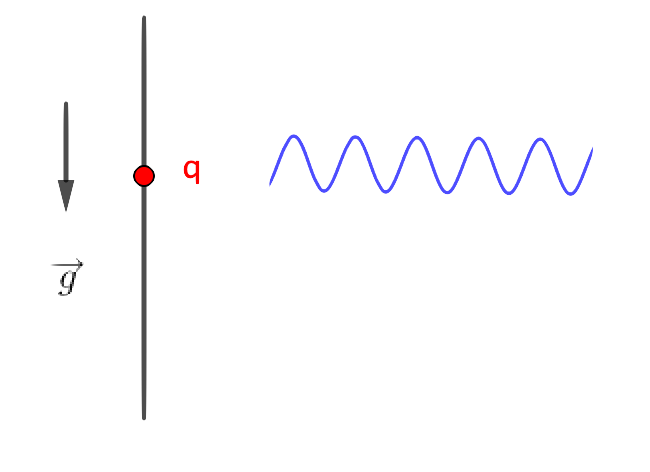
\includegraphics[width=.35\textwidth]{imagenes/img07-01.png}
	\end{figure}
	Partícula $\ q,\ m \ $ que se puede desplazar libremente en una recta, en presencia de la gravedad y ante un campo electromagnético (radiación en forma de onda plana).
	
	El lagrangiano del sistema es:
	
	$$L = \dfrac m 2 \dot z^2 - (qA_o-q\vec v \cdot \overrightarrow A) - mgz$$
	\end{multicols}
\end{example}

Para este tipo de problemas sería más adecuado usar el formalismo \emph{hamiltoniano} que el 	\emph{lagrangiano}. Lo veremos en próximos capítulos.

\subsection{Acoplamento mínimo}

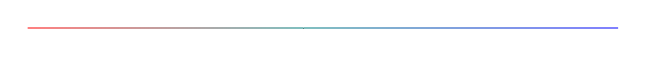
\begin{tikzpicture}
	\fill [left color=red!50, right color=teal!50] (0,0) rectangle (3.5,.01);
	\fill [left color=teal!50, right color=blue!50] (3.5,0) rectangle (7.5,.01);
	\end{tikzpicture}
\vspace{0.5cm}


Supongamos una carga libre en presencia de un campo electromagnético (radiación), solo va a haber fuerza de Lorentz.

En estas ocasiones, lo veremos más adelante (formulación hamiltoniana) pero es conveniente recordarlo, la cantidad de movimiento definida como $\ \vec p = m \vec v \ $ no es la manera adecuada de definirla, hay que usar la forma:

$$\boxed{ \ \boldsymbol{ \overrightarrow {\mathcal P} \ = \ m\vec v \ + \  q\overrightarrow A} \ }$$